\chapter{Tests}

This chapter describes the different tests that were performed to verify the
correctness and reliability of the system.
Both automated and manual tests
were conducted in order to evaluate the functionality, stability, and
performance of the application.

\section{Unit Tests}
Unit tests were implemented for both the client and the server
components of the system.
Table~\ref{tab:unit-test-overview} shows an overview of the Unit tests for server and client.

\begin{table}[h]
    \center

    \begin{tabular}{|p{4cm}|p{6cm}|p{6cm}|}
        \hline
        \textbf{Characteristic} & \textbf{Client} & \textbf{Server} \\
        \hline
        \textbf{Technology} & Vitest & Pytest for Python~3.14.3 \\
        \hline
        \textbf{Included filetypes} & \texttt{.ts} & \texttt{.py} \\
        \hline
        \textbf{Main tested components} & ViewModels, Service Implementations, Local Data Caching & Service Endpoints, Managers and Persistence Repositories \\
        \hline
        \textbf{Test Count} & 176 & 227 \\
        \hline
        \textbf{Line Coverage} & 76.79\% & n.a. \\
        \hline
        \textbf{Statement Coverage} & 76.79\% & 94\% \\
        \hline
        \textbf{Branch Coverage} & 86.9\% & 83\% \\
        \hline
        \textbf{Function Coverage} & 84.83\% & n.a. \\
        \hline
    \end{tabular}

    \caption{Unit Test Overview}
    \label{tab:unit-test-overview}
\end{table}

\subsection{Adittional Notes}
\subsubsection{Client}
Missing coverage in the client is mostly generated in ViewModels, where edge-cases that require
very specific user-input are not simulated.
Configuration files, as well as test helper are automatically excluded from the coverage statistics.

\subsection{Server}
To simplify testing, a central test bootstrap was implemented in
\texttt{tests/conftest.py}.
This configuration provides default environment
settings and lightweight dependency stubs, allowing the tests to run without
requiring external services.

Lower coverage values mainly originate from modules that interact with
external systems, including the application bootstrap code, vector database
initialization modules, graph generation internals, the OpenAI client
transport layer, and validator subprocess logic.

During test execution, minor warnings are emitted regarding the configured
JWT secret length and resource cleanup during SQLite teardown. These warnings
do not affect the correctness of the test results.

\section{User Tests}

\subsection{General Procedure}

Several user tests were conducted to evaluate the usability of the application.
Participants were asked to perform typical workflows within the system.
These tasks included logging in, creating and managing conversations, and
interacting with the system's functionality, which involves communication
between the client interface and the server backend.

Overall, all participants were able to successfully complete the assigned tasks.
Most users quickly understood the basic functionality of the system and were
able to operate the application without major difficulties.
However, some
uncertainties occurred at certain points, where minor assistance was occasionally
required.

The navigation within the application was generally perceived as intuitive.
In particular, creating new conversations and sending requests worked without
additional explanations in most cases.
The display of responses and the
structure of the conversation view were also quickly understood by the test
participants.

Some uncertainties arose in specific dialogs or settings.
In a few cases,
it was not immediately clear which action a certain button triggered or what
input was required.
These issues were usually resolved quickly after a short
explanation.

In summary, all participants were able to complete the intended tasks
successfully.
The overall operation of the application was generally described
as understandable and logically structured.

\subsection{User Ratings}

After completing the tasks, the participants were asked to evaluate the
application based on several criteria.
The following aspects were considered:

\begin{itemize}
    \item Clarity of the user interface
    \item Ease of navigation
    \item Application performance
    \item Understandability of error messages
    \item Overall usability
\end{itemize}

The ratings were predominantly in the range of \textit{good} to \textit{very good}.
In particular, the clear structure of the interface and the fast response time
of the application were highlighted positively.

Potential improvements were mainly identified in the clarity of certain dialogs
and in the recognizable of some interactive elements.

\section{End-to-End Tests}
In \textit{End-to-End} Tests (E2E-Tests), the whole system is tested without any mocked dependencies.
This is realized by automatically simulating user-input in the browser using an E2E-Agent, in our case \textit{Playwright}.

The following table gives an overview which of the test cases presented during the \textit{Requirements Analysis} have been realized as E2E-Tests.

\begin{table}[h]
    \center

    \begin{tabular}{|p{3cm}|p{4cm}|p{6cm}|}
        \hline
        \textbf{Test Case} & \textbf{Status} & \textbf{Additional Notes} \\
        \hline
        $\langle$ \textit{T10} $\rangle$ & Not implemented & Automatic login with Google OAuth provider not possible due to captcha requirements. \\
        \hline
        $\langle$ \textit{T20} $\rangle$ & Implemented & \\
        \hline
        $\langle$ \textit{T30} $\rangle$ & Partially Implemented & Verification of email not possible \\
        \hline
        $\langle$ \textit{T40} $\rangle$ & Implemented & \\
        \hline
        $\langle$ \textit{T50} $\rangle$ & Implemented & \\
        \hline
        $\langle$ \textit{T60} $\rangle$ & Implemented & \\
        \hline
        $\langle$ \textit{T70} $\rangle$ & Implemented & \\
        \hline
        $\langle$ \textit{T80} $\rangle$ & Implemented & \\
        \hline
    \end{tabular}

    \caption{Unit Test Overview}
    \label{tab:e2e-test-overview}
\end{table}

\section{Server Load Tests}
In the server load-tests, the server is tested under a large and growing amount of users.
The purpose of these tests is to observe the behavior under load, finding an upper bound on which the server can comfortably run and to check, if after a period of high request, the server returns back into a stable state.

\subsection{Device Specs}
The setup and physical device stats play a large role in the result of the load tests.
The results presented were performed on a machine with the following stats:

\begin{itemize}
\item \textbf{CPU:} Intel Pentium G4400T @ 2.90\,GHz (2 cores)
\item \textbf{Memory:} 15\,GB RAM
\item \textbf{Storage:} 476.9\,GB NVMe SSD (system disk)
\item \textbf{Operating System:} Debian GNU/Linux 13 (Trixie)
\item \textbf{Kernel:} 6.12.63+deb13-amd64
\end{itemize}

The server runs on the machine described above. Load tests were executed from a separate machine located in a different network.

\subsection{Test Structure}
Several different simulations with each different scenarios were created to test different parts of the isolated server.
Simulations were independently performed for the parts:

\begin{itemize}
    \item Server Settings (Quota and Analytics)
    \item LLM Configuration
    \item Authentication
    \item Conversations and Messages
\end{itemize}

\subsection{Request Structure}
The requests were structured in a ramp-up model: 
This configuration increases the number of virtual users sending requests to the system. It starts with 1 user per second and increases the rate by 1 additional user per second at each step. There are 3 steps in total, and each step runs for 3 seconds. In other words, the test runs 1 user/sec for 3 seconds, then 2 users/sec for 3 seconds, and finally 3 users/sec for 3 seconds.

As mentioned above, this request structure was created specifically for the hardware and shouldn't be used globally.

\subsection{Test Results}
The response times, shown in \ref{fig:resp_settings}, \ref{fig:resp_llms}, \ref{fig:resp_auth}, and \ref{fig:resp_conv} display a clear pattern of different average response times.

This highly correlates with the amount of sql/vector/llm access that has to be done, which is low in the settings and llm-model simulation, medium in the authentication simulation and high in the conversation simulation.

Failing (i.e. non-responded requests) in the conversation simulation stem from timeouts and cancelled responses by the server, due to overload.

Figure \ref{fig:active-users} and \ref{fig:influx-users} show the total and increase of simulated virtual users.

The verbose and complete load-test result is included in the appendix as several html-files

\begin{figure}
    \centering
    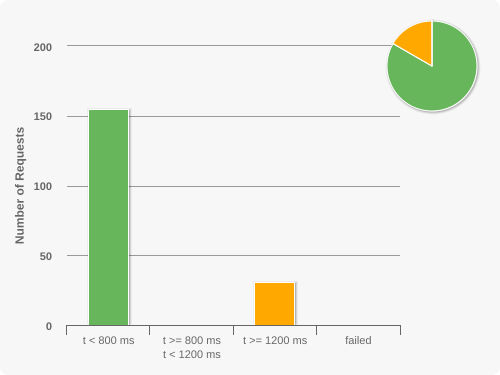
\includegraphics[width=0.5\linewidth]{figures/set}
    \caption{Response Times for Settings Simulation}
    \label{fig:resp_settings}
\end{figure}

\begin{figure}
    \centering
    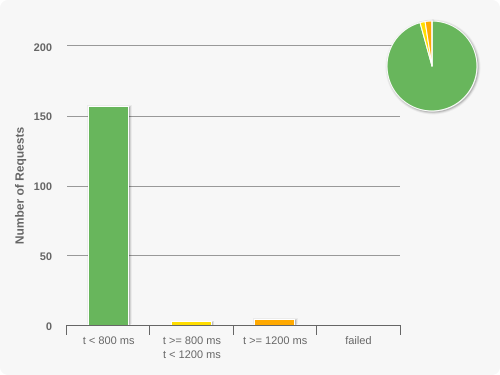
\includegraphics[width=0.5\linewidth]{figures/llm}
    \caption{Response Times for LLM-Model's Simulation}
    \label{fig:resp_llms}
\end{figure}

\begin{figure}
    \centering
    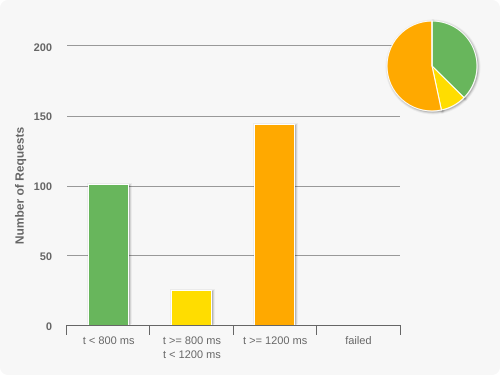
\includegraphics[width=0.5\linewidth]{figures/auth}
    \caption{Response Times for Authentication Simulation}
    \label{fig:resp_auth}
\end{figure}

\begin{figure}
    \centering
    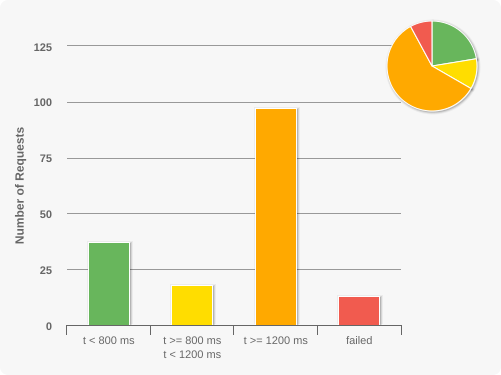
\includegraphics[width=0.5\linewidth]{figures/conv}
    \caption{Response Times for Conversation Simulation}
    \label{fig:resp_conv}
\end{figure}


\begin{figure}
    \centering
    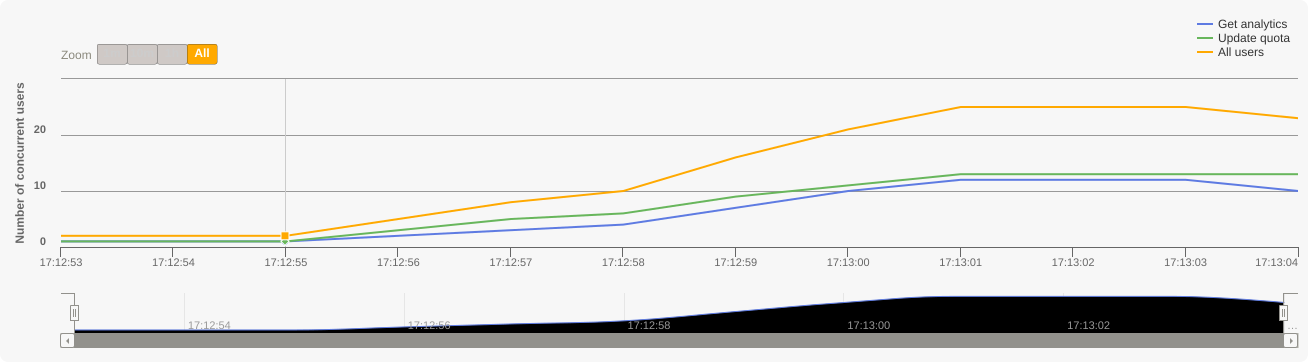
\includegraphics[angle=90,height=20cm]{figures/users}
    \caption{Total active users, Settings scenario}
    \label{fig:active-users}
\end{figure}

\begin{figure}
    \centering
    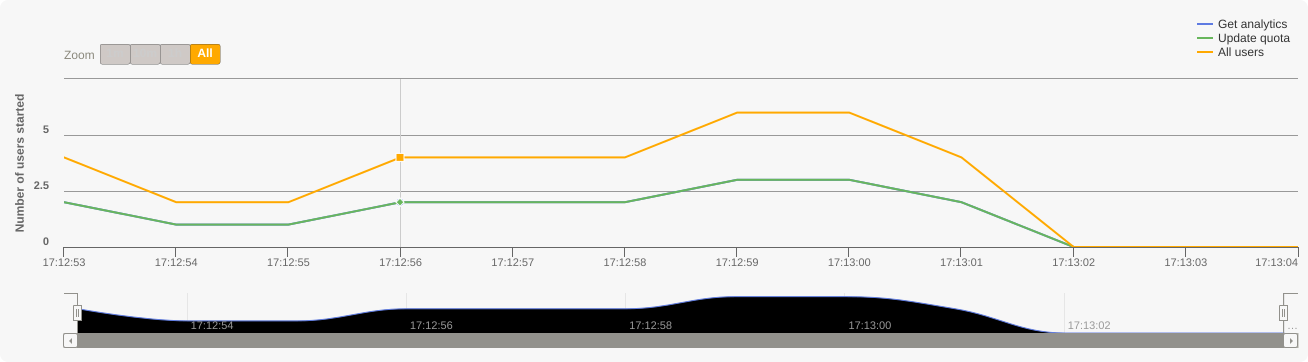
\includegraphics[angle=90,height=20cm]{figures/users_started}
    \caption{Total starting users, Settings scenario}
    \label{fig:active-users}
\end{figure}